%%
%% 研究報告用スイッチ(情報処理学会用ファイルをEC2014用に変更)
%% [techrep]
%%
%% 欧文表記無しのスイッチ(etitle,jkeyword,eabstract,ekeywordは任意)
%% [noauthor]
%%

\documentclass[submit,techreq]{ec2014}
%\documentclass[submit,techreq,noauthor]{ipsj}


\usepackage[dvips]{graphicx}
\usepackage{latexsym}

\def\Underline{\setbox0\hbox\bgroup\let\\\endUnderline}
\def\endUnderline{\vphantom{y}\egroup\smash{\underline{\box0}}\\}
\def\|{\verb|}

\setcounter{巻数}{54}%vol53=2012
\setcounter{号数}{10}
\setcounter{page}{1}


\begin{document}


\title{笑い声呈示により自然な笑顔を撮影するカメラの提案}
\etitle{How to Prepare Your Paper for IPSJ Journal \\
(version EC2014)}

\affiliate{UTokyo}{東京大学\\
UTokyo, 7-3-1, Hongo, Bunkyo-ku, Tokyo}

\author{伏見 遼平}{Ryohei Fushimi}{UTokyo}[fushimi@nae-lab.org]
\author{福嶋 政期}{Shogo Fukushima}{UTokyo}[shogo@nae-lab.org]
\author{苗村 健}{Takeshi Naemura}{UTokyo}[naemura@nae-lab.org]

\begin{abstract}
記念撮影で自然な表情を撮影するのは難しい.本研究では被撮影者に自然な笑顔の表出を促すカメラを検討している.本稿では笑い声が笑顔や笑いを誘発する現象に着目し,シャッターを切る前に笑い声を再生することで自然な笑顔を撮影するカメラシステムを提案する.効果を検証するために,シャッター音・笑い声(青年)・笑い声(幼児)の3条件で表情の変化を比較した.さらに笑い声呈示から表情表出までの時間差に着目しシャッターを切るタイミングを検討した.
\end{abstract}


%\begin{jkeyword}
%情報処理学会論文誌ジャーナル,\LaTeX,スタイルファイル,べからず集
%\end{jkeyword}
%
\begin{eabstract}
This document is a guide to prepare a draft for submitting to IPSJ
Journal, and the final camera-ready manuscript of a paper to appear in
IPSJ Journal, using {\LaTeX} and special style files.  Since this
document itself is produced with the style files, it will help you to
refer its source file which is distributed with the style files.
\end{eabstract}

%\begin{ekeyword}
%IPSJ Journal, \LaTeX, style files, ``Dos and Dont's'' list
%\end{ekeyword}




\maketitle

%1
\section{はじめに}

カメラは被写体のありのままの姿を記録するためにデザインされている.ストロボなどを除けば、基本的にはカメラや付属する機器は被写体に対して働きかけを行うものは少ない.しかし、ポートレートなどの人物写真については、被写体となる人間とのコミュニケーションも重要である.カメラマンからは「ハイチーズ」「笑って」などの声掛けがなされるが,言語でコミュニケーションを取ったり,笑顔を作るように誘導したとしても,随意的な笑顔しか撮影することができない.自然な笑顔

% (「自然な笑顔」ぼくたちが自然な笑顔をどういうものだと思っているかを示す.ハイチーズみたいな笑い方,自然な表情であるかは微妙.イラストでこれやりたいが分かる2枚)

本研究では、被写体にカメラそのものが働きかけ、笑顔を誘発するようなカメラシステムを研究する.笑顔を誘発するために,つられ笑いや思い出し笑いなどの非随意的なメカニズムを使えば,自然な笑顔が撮影できるはずである.中でも本論文では、笑い声が笑いを誘発する効果を利用して、シャッターを切る前に笑い声を再生することで自然な笑顔を撮影するカメラシステムを提案する.また,システムをスマートフォン上で動作するアプリケーションとして実装し,実際に効果を検討する.

まず,予備実験として笑顔を誘発しやすい笑い声音声を検討する.次に実験室の統制された環境で,2種類の笑い声音声と通常のシャッター音で撮影された笑顔にどのような違いがあるかを調べる.最後に,スマートフォンアプリとして配布し,実際の記念撮影のシチュエーションでどのような写真が撮影できたかを調べる.

\begin{figure}[h]
\begin{minipage}{0.49\columnwidth}
\begin{center}
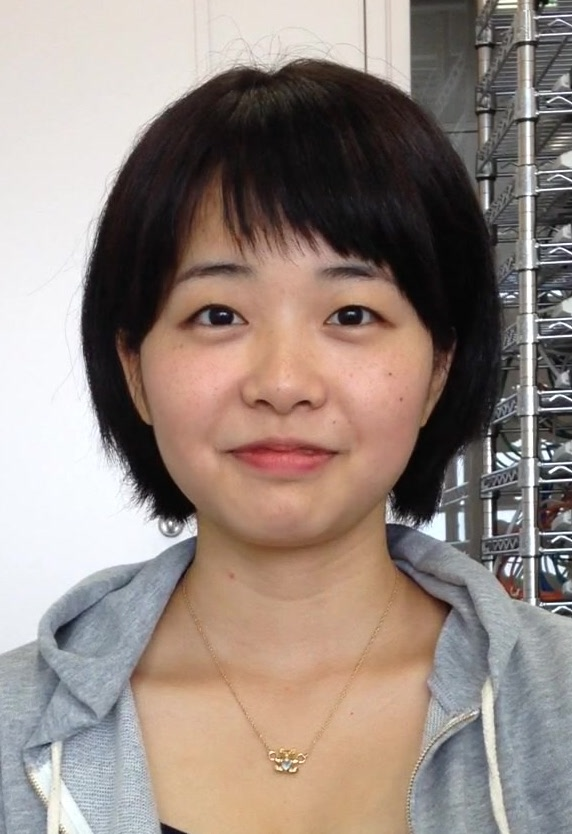
\includegraphics[width=35mm, bb=0 0 572 834]{images/cap_28.jpg}
\caption{「笑って」の笑顔}
\end{center}
\end{minipage}
\begin{minipage}{0.49\columnwidth}
\begin{center}
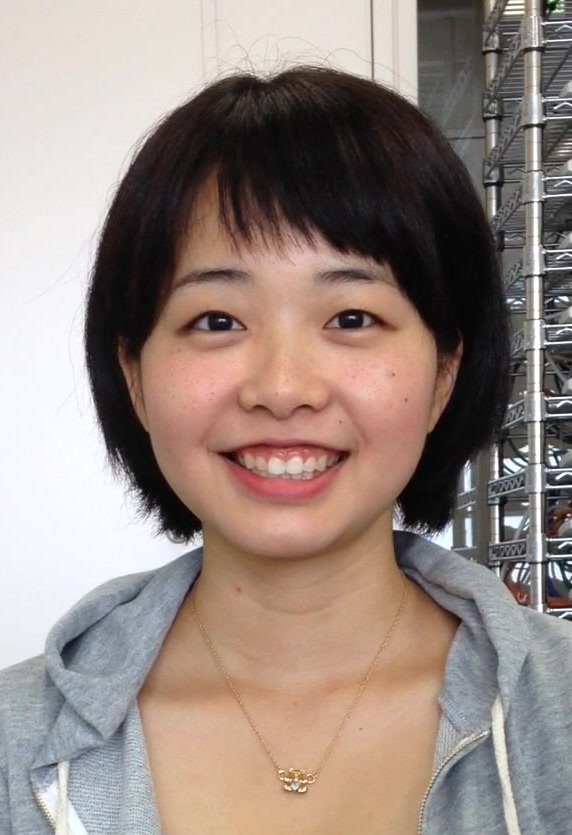
\includegraphics[width=35mm, bb=0 0 572 834]{images/cap_123.jpg}
\caption{自然な笑顔}
\end{center}
\end{minipage}
\end{figure}



%2
\section{関連研究}
\subsection{カメラ側からのインタラクション (自然な表情を取るための試み)}
本研究は,写真撮影のシーンにおける,カメラと被撮影者の間の非随意的・非言語的インタラクションとして位置づけることができる.

まず,被写体への光学的な働きかけとして,照明を用いて被写体を明るくみせるストロボが代表的である.キセノンランプやLEDを用いたストロボは多くのカメラデバイスに搭載されている.レフ板を用いて環境光を反射させて被写体にあてることも写真撮影には一般的である.人物写真においてはこれに加えて,瞳が表情の印象に影響を与えることから,ポートレート写真撮影ための書籍やWebサイトでは,被写体のまわりに照明や白いレフ板や布を置いてこれらの光を瞳に写しこむキャッチライトというテクニックが紹介されている.

次に,被写体への言語的なインタラクションについて整理する.記念撮影のシーンにおいてカメラマンによる被写体への語りかけや掛け声が多くみられ,これには位置やポーズ,表情についての指示だけではなく,被撮影者をリラックスさせようという意図の語りかけも多く見られる.言語的アプローチは非撮影者に表情の指示を伝えることができる点で有効だが,これは随意的な笑顔しか撮影できない.トークなどを通じて非随意的な笑いを意識して引き出すことのできるカメラマンも存在するが,簡単ではない.「チーズ」「ミッキー」などの語末に /i/ 音がある単語を発音させ,口角を上げさせる撮影の手法もある.またプリクラ撮影機では,具体的なポーズの指示について,事前収録された音声が再生されるが,インタラクティブ性はない.

\begin{figure}[h!]
  \centering  
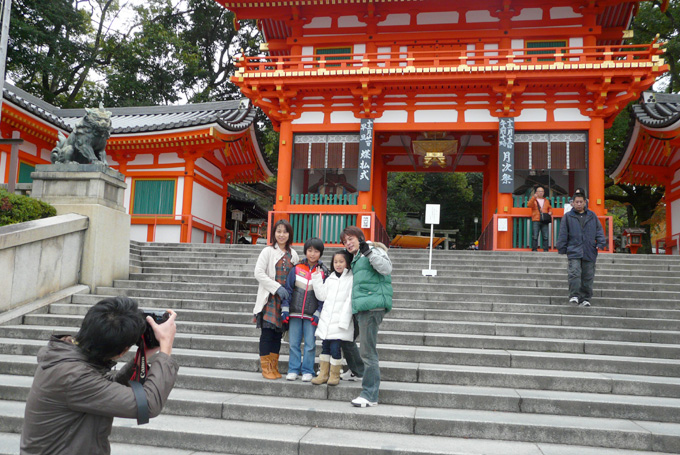
\includegraphics[width=70mm, bb=0 0 680 455]{images/murataphoto-main.jpg}
\caption{プロカメラマンの写真撮影の例}
  \label{recursive}
\end{figure}






最後に,非言語的アプローチについてまとめる.D2Cのリリースしたスマートフォン向けアプリ「笑顔が撮れる こどもカメラ」は,幼児の自然な笑顔を写真におさめるためのアプリケーションである.スマートフォンの画面にキャラクターを表示させ,これを動かすことで幼児の興味を引き,シャッターを切る.これは用途を子供向けに限定しており,視覚的アプローチを取るものであるが,本研究には最も近い事例である.

%% ※ 表

\subsection{笑い声呈示による笑い誘発}

笑い声の伝染現象は古くから研究されている.Provineは,心理学の講義を履修した128名の学生に対し,18秒間の笑い声を聞かせ,42秒間の間を空けることを10回繰り返し,それぞれの試行について笑顔になったか否かおよび笑ったか否かを報告させた.繰り返しにより笑顔・笑いを誘発できた割合は大きく下がり,繰り返しの後半では不快感を感じたという報告も多かった. [Provine, 1992] 

笑い声は音声・映像コンテンツに対する刺激の重畳としても用いられる (ラフトラック).映像コンテンツに対して ... らは,多い方は 社会的に近い集団による笑い声の方が,そうでない集団の笑い声よりも笑いの伝染を引き起こしやすいことを … らは指摘している.
 最後に,笑い誘発を実世界のデバイスに応用した例について取り上げる.「くすぐりエルモ (Tickle me Elmo)」は,子供に人気のキャラクター「エルモ」のぬいぐるみであるが,腹部を触るとエルモが笑い転げる.

\section{システム}

本システムでは,笑い声を非撮影者に呈示しながら写真を撮影する必要がある.一眼レフなどのデジタルカメラのシャッターと同期して音声を再生する装置を検討したが,同期のための機構を特別に必要となってしまう.同期を簡便に実現でき,音声再生から撮影までの遅延を自由に制御できるという利点を持つスマートフォン向けのアプリケーションとして実装することとした.

\begin{figure}[h!]
  \centering  
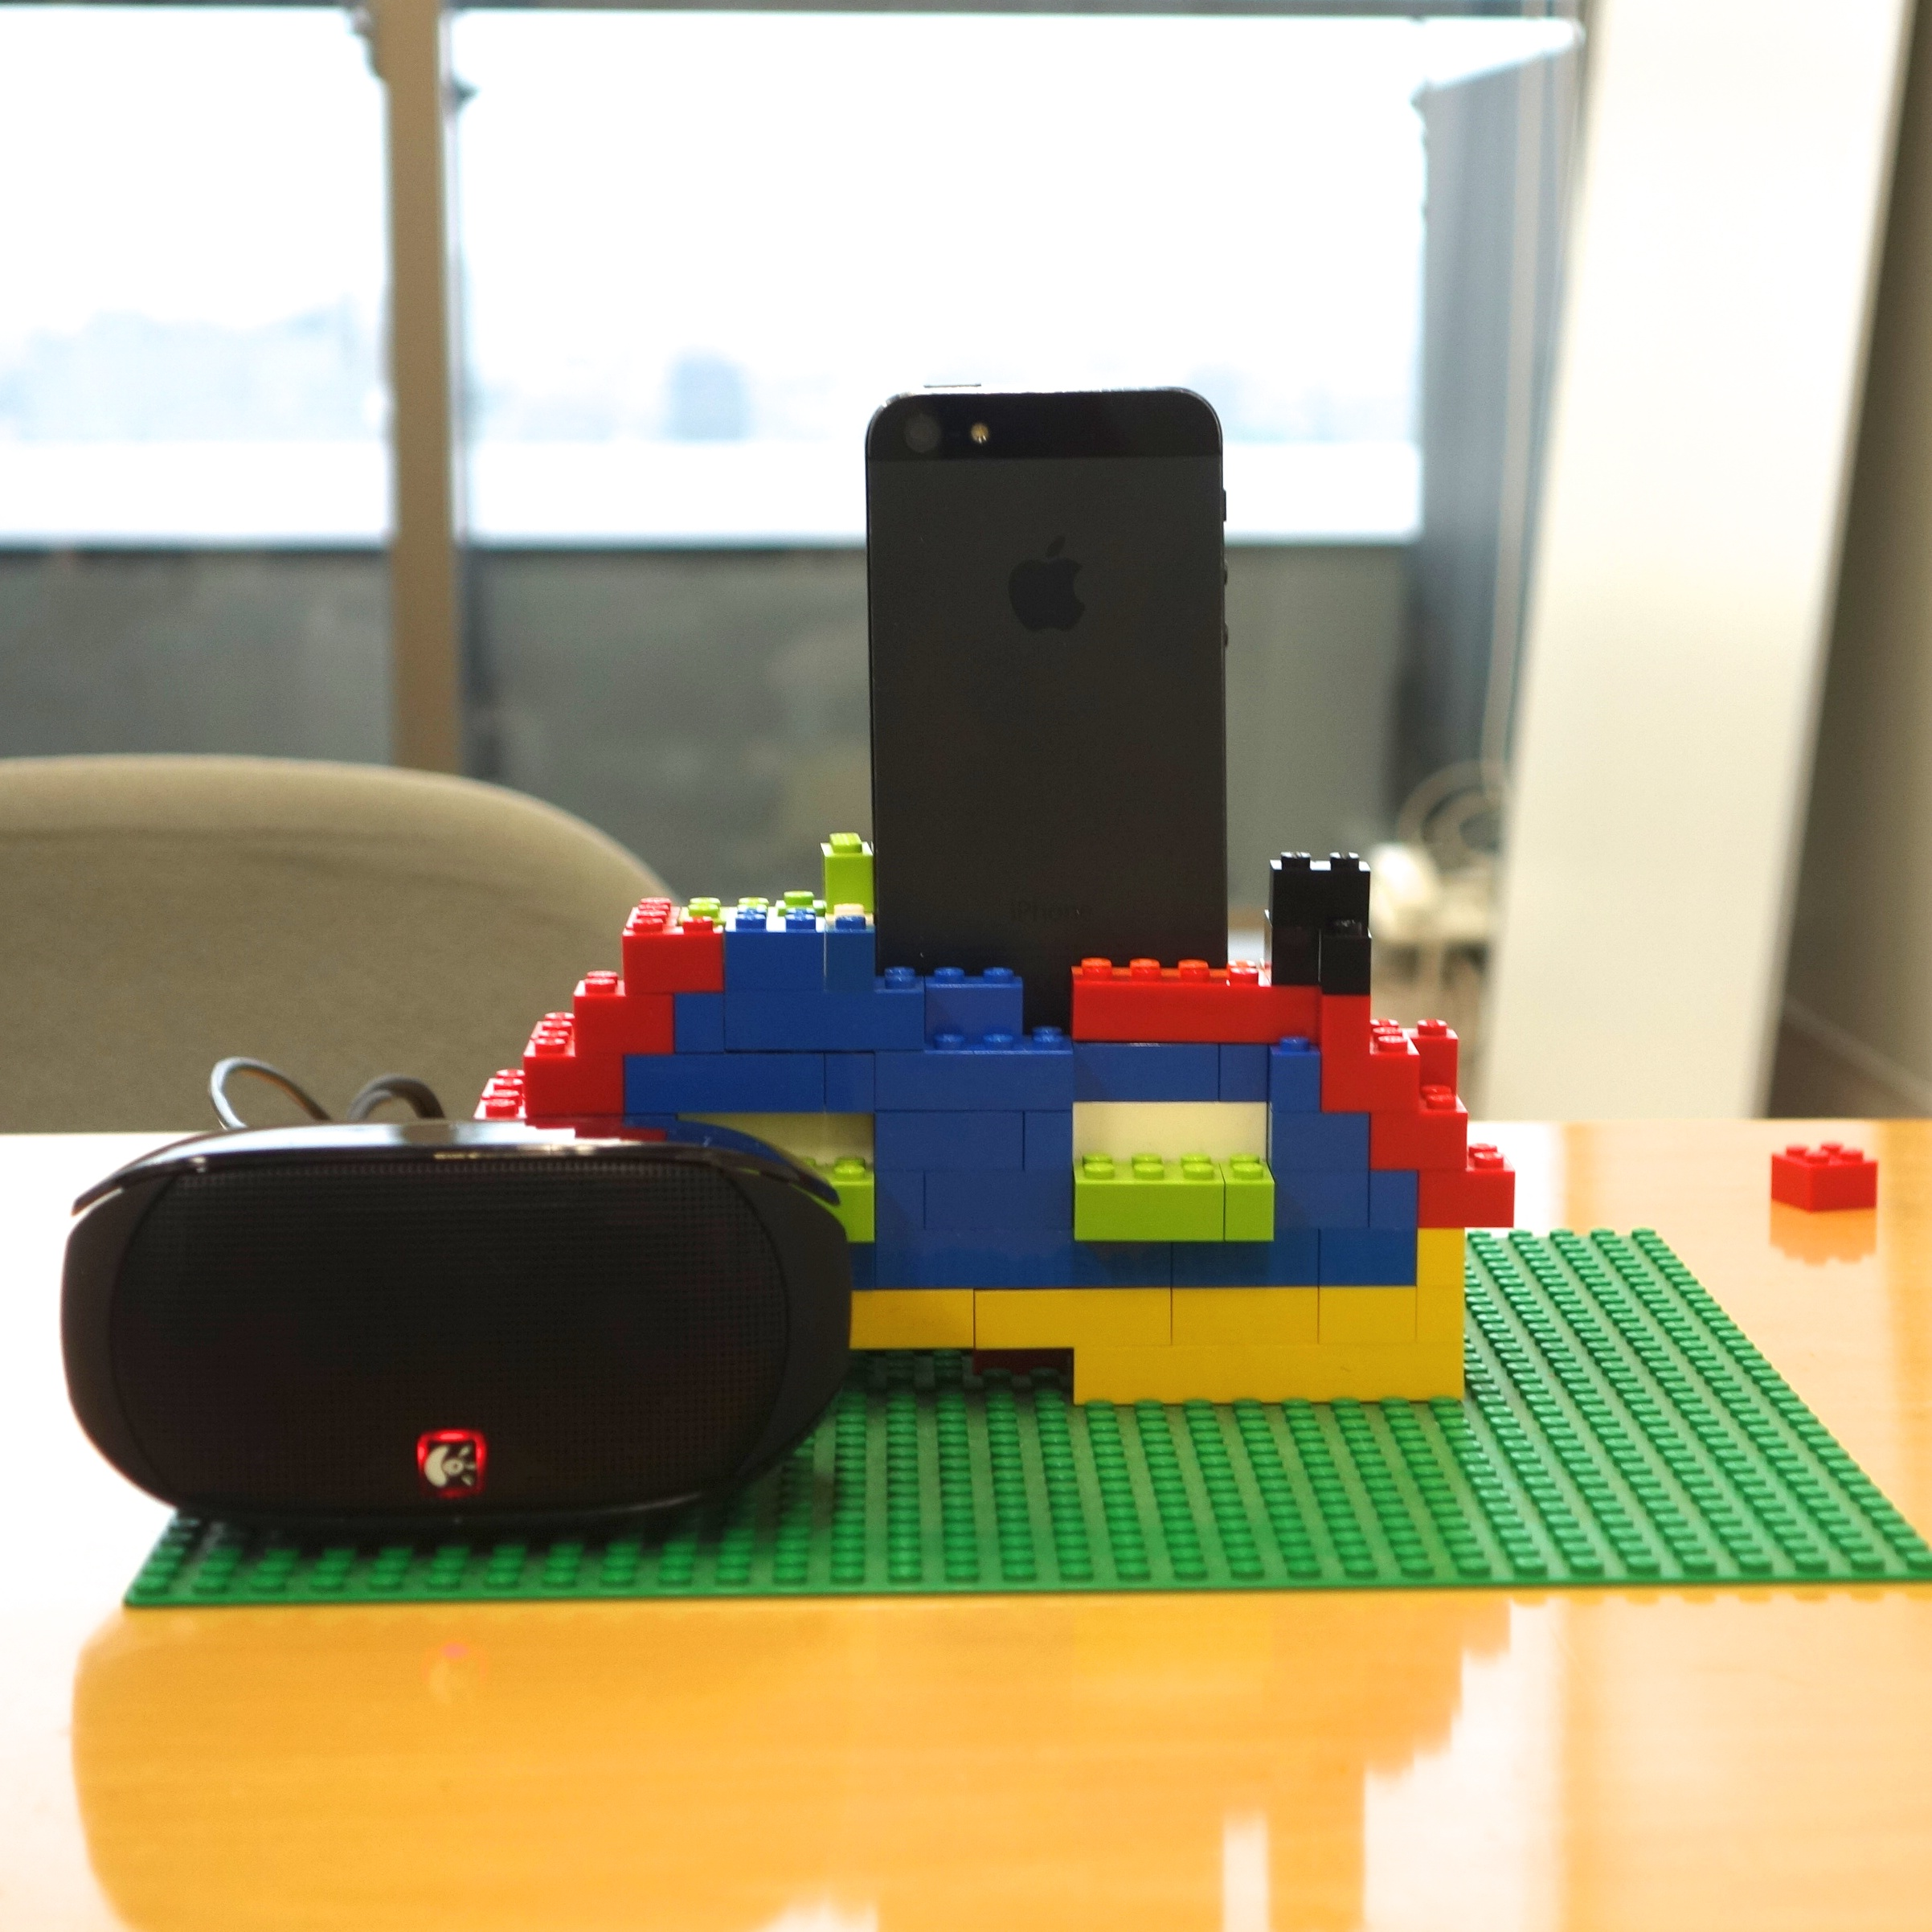
\includegraphics[width=55mm, bb=0 0 2404 2404]{images/system.jpg}
\caption{実装したシステム}
  \label{recursive}
\end{figure}

本システムはスマートフォン,スピーカによって構成されている.ボタンを押した時刻から録画を始め,タイマーで,音声を再生し,録画をストップするアプリケーションをObjective-Cで記述し,iOSのスマートフォンにインストールした.アプリケーションは通常の写真撮影モードと,動画撮影するモードがある.また,著者以外でも実験ができるように,教示をアプリケーションの画面の中に埋め込んだ.
\begin{figure}[h]
\begin{minipage}{0.49\columnwidth}
\begin{center}
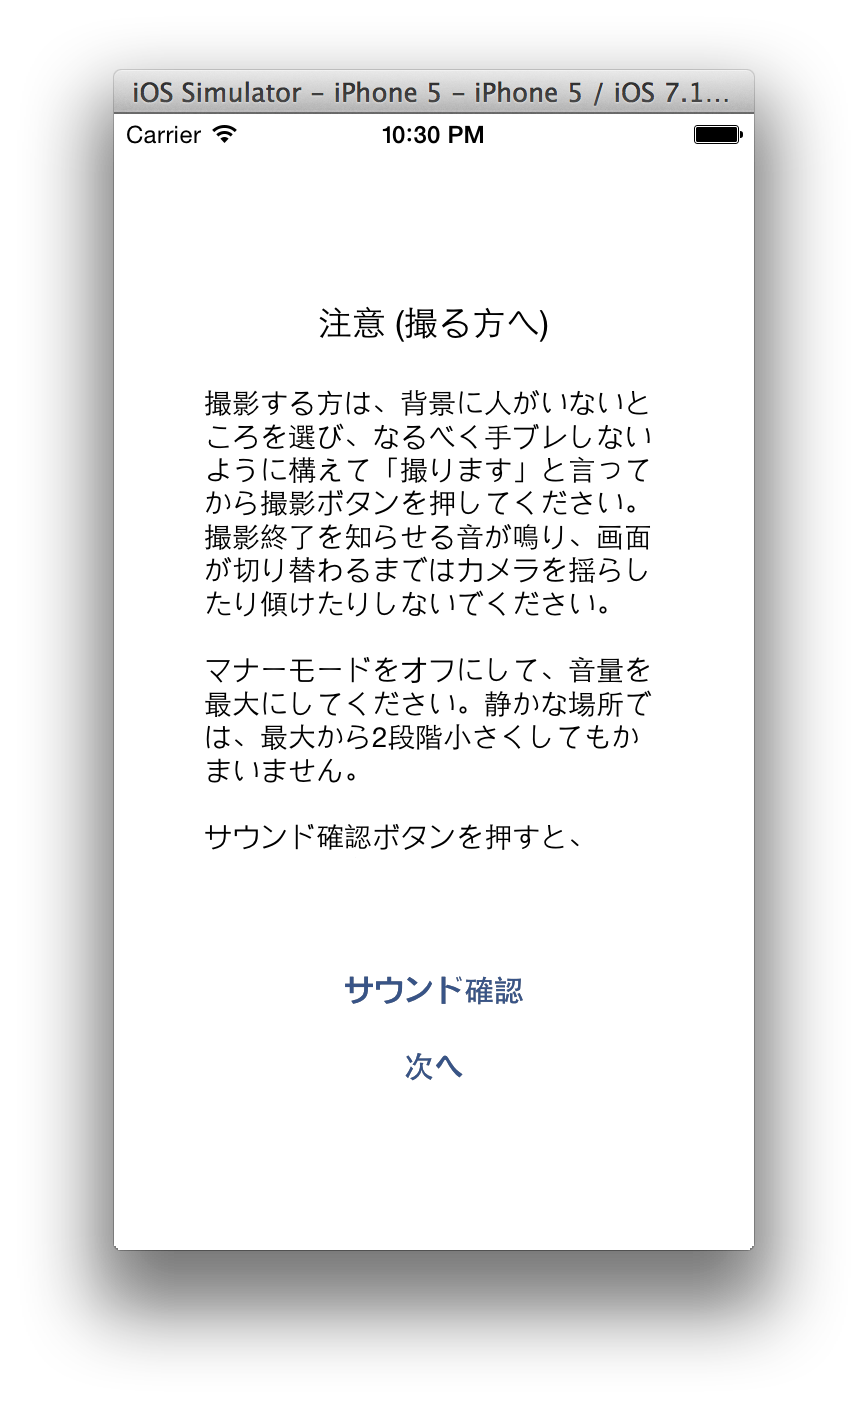
\includegraphics[width=35mm, bb=0 0 434 704]{images/ss/ss1.png}
\caption{スクリーンショット}
\end{center}
\end{minipage}
\begin{minipage}{0.49\columnwidth}
\begin{center}
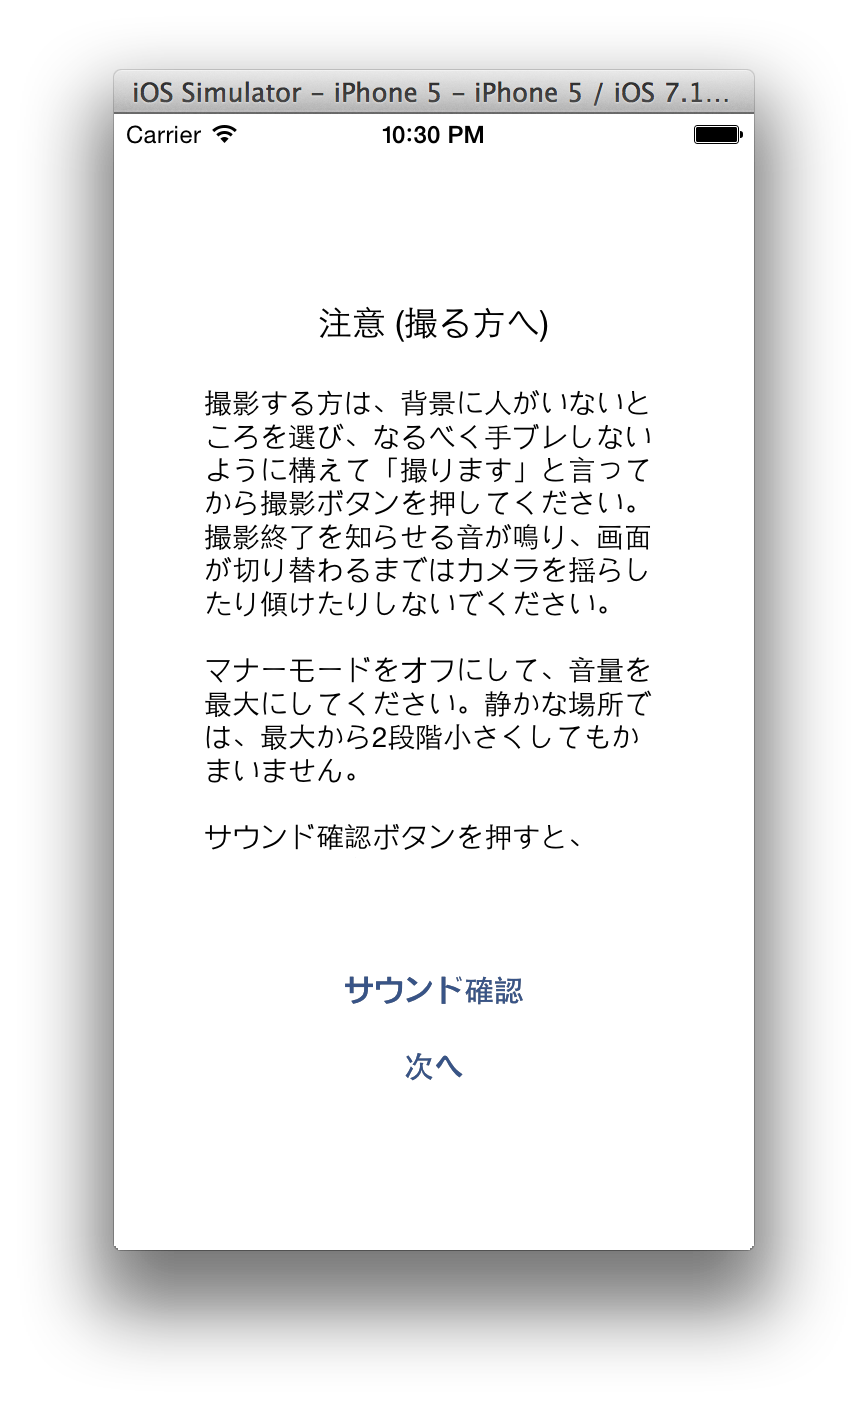
\includegraphics[width=35mm, bb=0 0 434 704]{images/ss/ss1.png}
\caption{スクリーンショット}
\end{center}
\end{minipage}
\end{figure}

\section{予備実験}

予備実験として,下記に示す5種類の笑い声を用意し,3人の被験者 (男性2名,女性1名) に聴かせた.笑顔を誘発する効果の大きかった (1)幼児の笑い声 (3)青年の笑い声を本実験に用いることにした.音声データはロイヤリティフリーの音声素材を提供するWebサイトaudioblocksから取得した.

\begin{enumerate}
 \item 幼児の笑い声
 \item 少年の笑い声
 \item 青年の笑い声
 \item 青年の3名の笑い声
 \item 多人数の笑い声(ラフトラック)
\end{enumerate}

感想として「5.は笑えない」

\section{実験1}
\subsection{目的}

本実験では,実験室において本システムが有効に

\subsection{実験条件および実験設備環境}

21-36歳の被験者19名に対して実験を行った.実験は静かな実験室で,実験者と二人の状況で行われた.実験条件として,音声を予備実験で選定した「青年の笑い声」「幼児の笑い声」「一眼レフカメラのオートフォーカス合焦音+シャッター音(対象条件)」に設定した3条件で実験を行った.カメラデバイスをスタンドに設置し,実験者はスタンドの右斜め後ろで被験者に教示を与えたのち,デバイスを操作した.

被験者の属性は東京大学・東京外国語大学の学生および東京大学の大学職員であった. (男性8名, 女性11名, 平均23.1歳) 

\begin{figure}[h!]
  \centering  
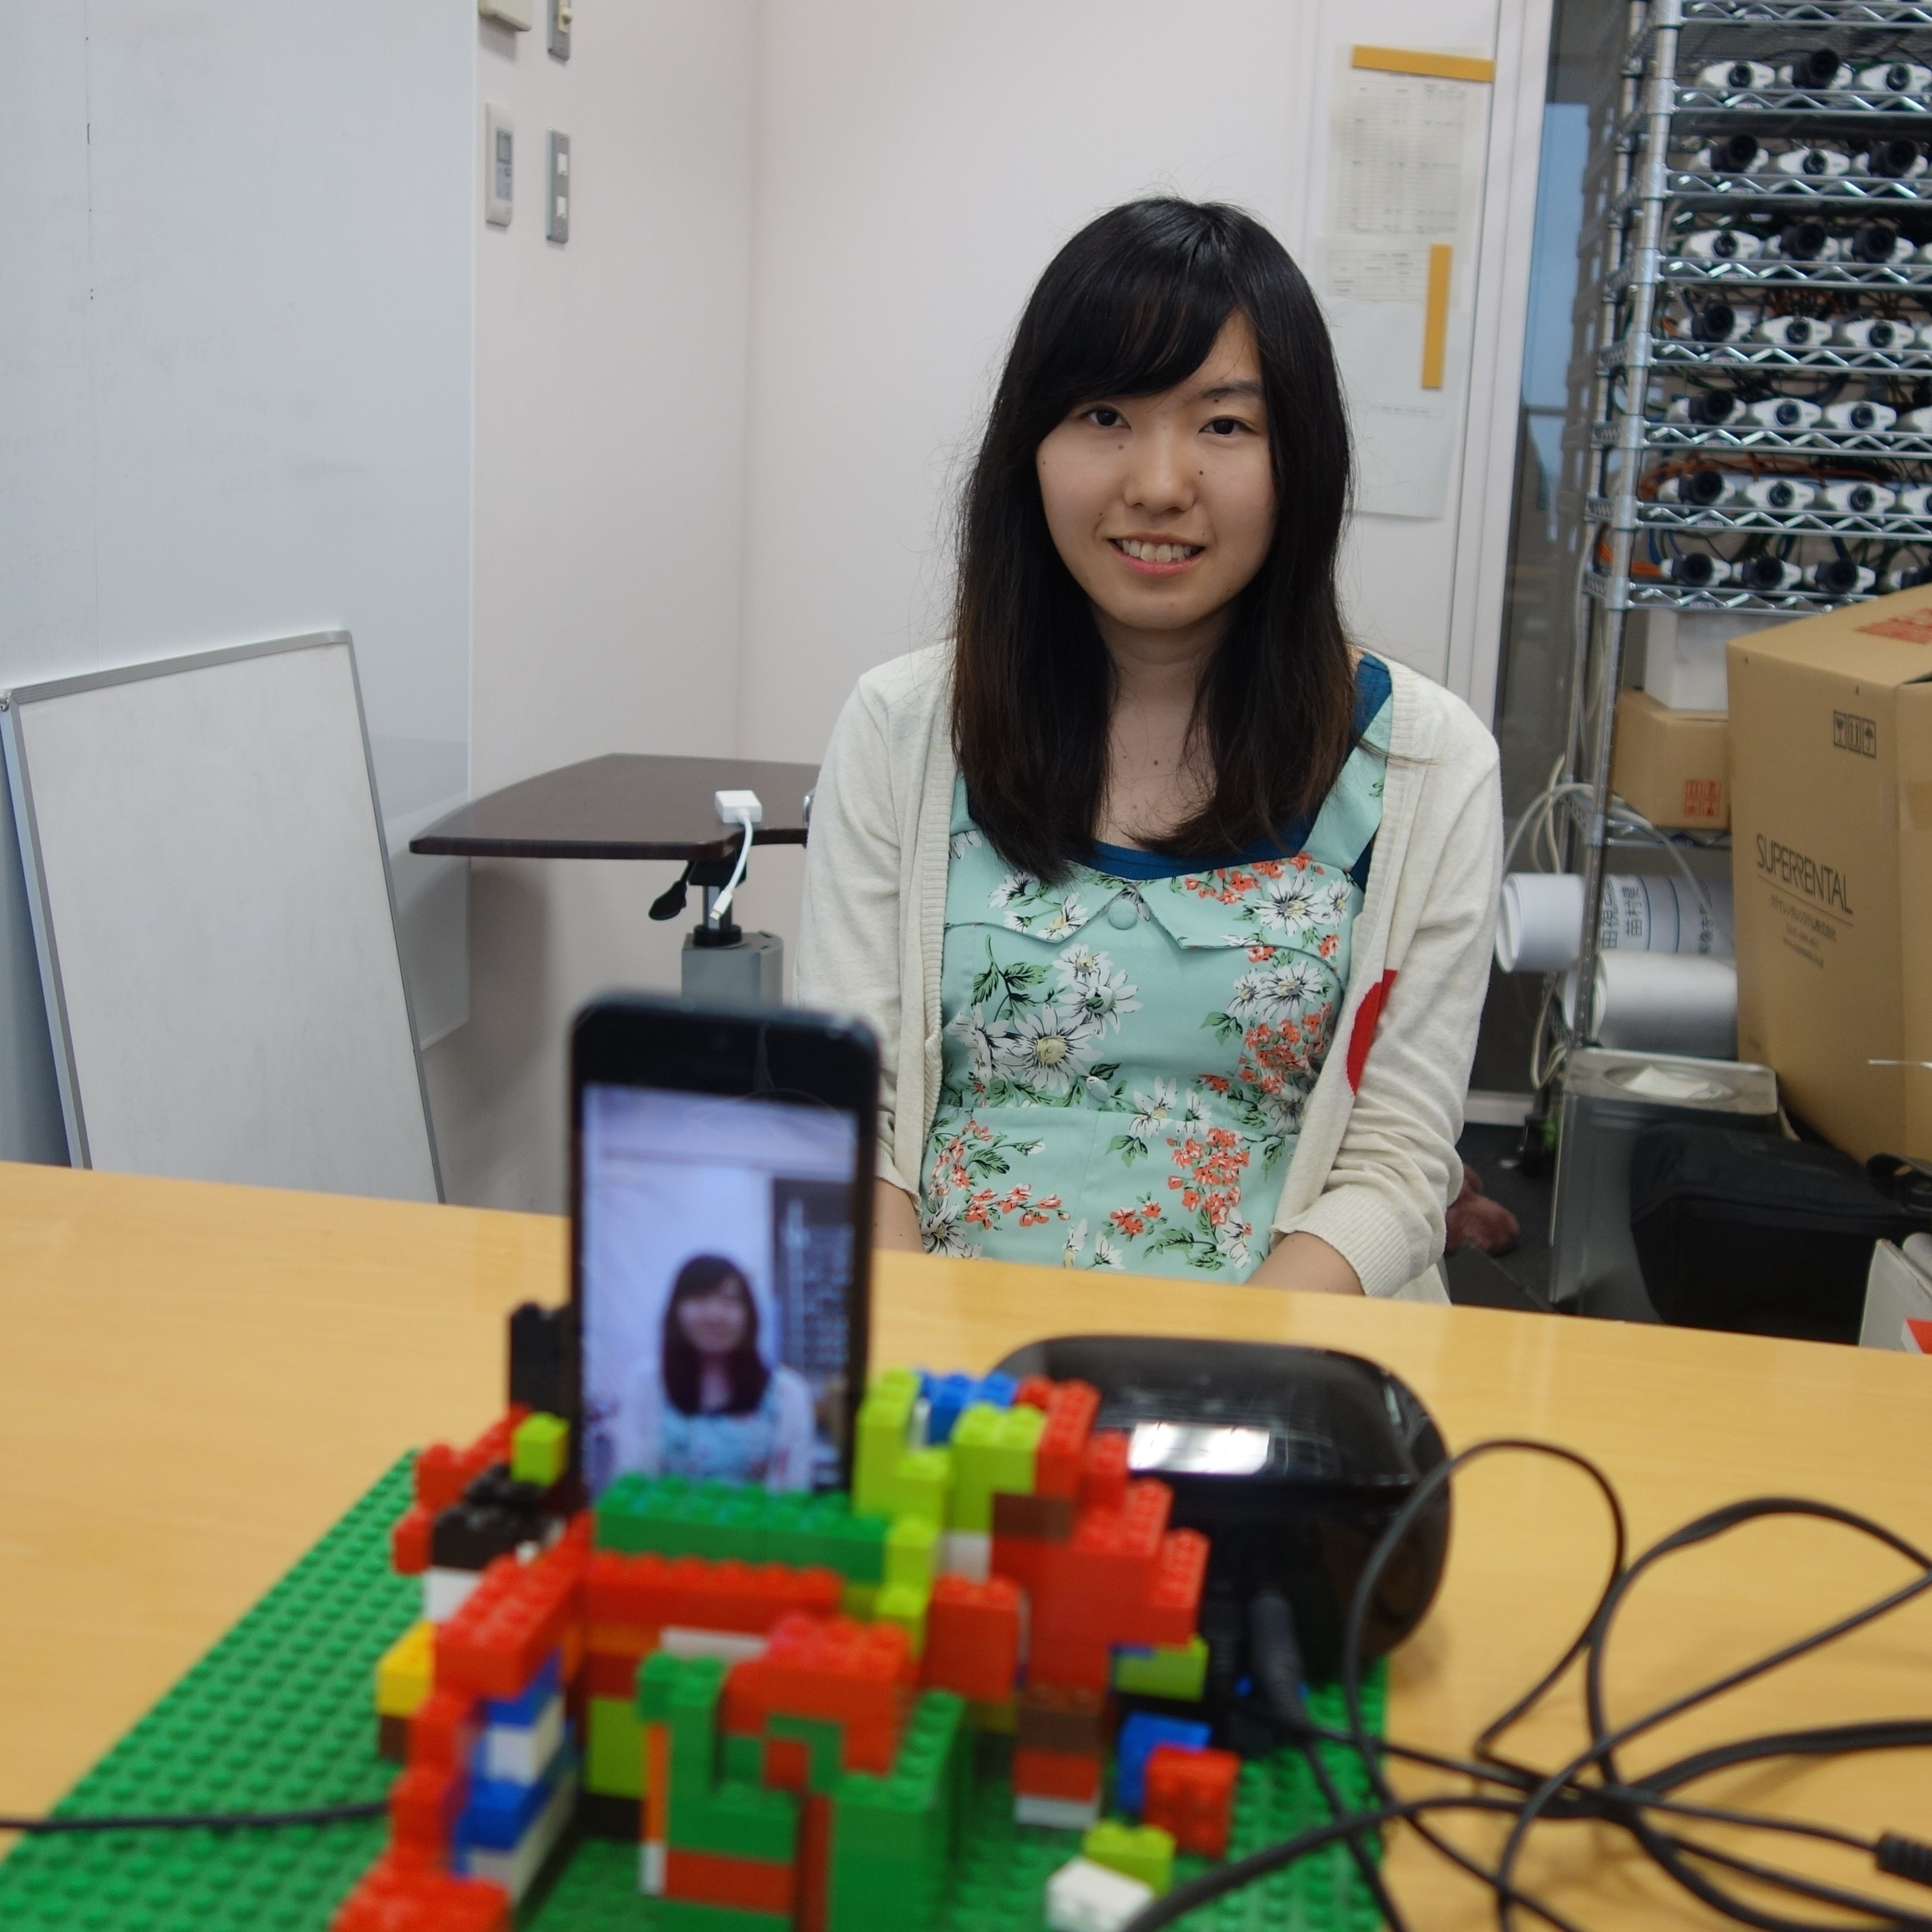
\includegraphics[width=55mm, bb=0 0 2312 2312]{images/DSC05173.jpg}
\caption{実験の様子}
  \label{recursive}
\end{figure}


\begin{table}[htb]
  \begin{center}
    \caption{実験条件}
    \begin{tabular}{|l|c|r||r|} \hline
      条件1 & 青年の笑い声 \\ \hline 
      条件2 & 幼児の笑い声 \\ \hline
      条件3 & 一眼レフカメラのAF合焦音+シャッター音 (対照) \\ \hline
    \end{tabular}
    \label{tab:price}
  \end{center}
\end{table}

\subsection{手続き}

被験者には,この実験は写真を撮る際のシャッター音の表情への影響を調べる実験であることが伝えられた.さらに注意としてシャッター音には長いものも短いものもあること,撮影中はなるべくカメラレンズを見つめるようにすることを伝えたのち,3条件で撮影を行った.順序効果を相殺するため,実験条件の順序はラテン方格法により割り当てられた.3条件すべての撮影後,それぞれの体験についてどういう感想を持ったかを聞いた.

\subsection{評価方法}

撮影された8秒間の動画から,15fpsで静止画像を切り出し,条件間の表情の差異,および表情の時間変化について分析を行った.

まず,Rekognition APIを用いて,各画像について笑顔尺度の測定を行った.Rekognition APIはOrbeus社による表情認識APIで,画像を送信すると映っている表情について笑顔尺度を解析し,0〜100の値で結果を返す.この値を顔全体の笑顔の度合いとみなし,値の時間変化と条件間の差異を分析した.

ただし,目を閉じている場合,笑顔尺度は目を閉じていない前後のフレームよりも大きく値が低下する.このことから,目を閉じていると判定されたフレームと,その前後2フレームについては,3フレーム前の笑顔尺度の値と,3フレーム後の笑顔尺度の値の平均値を採用した.

\subsection{結果}

笑顔尺度の時間変化を条件ごとに平均した値をプロットしたものを図\ref{graph-smooth}に示す.音声が流れ始めてすぐは全く変化がなく,1.0秒ごろから笑顔度に条件間の差が認められる.

\begin{figure}[h!]
  \centering  
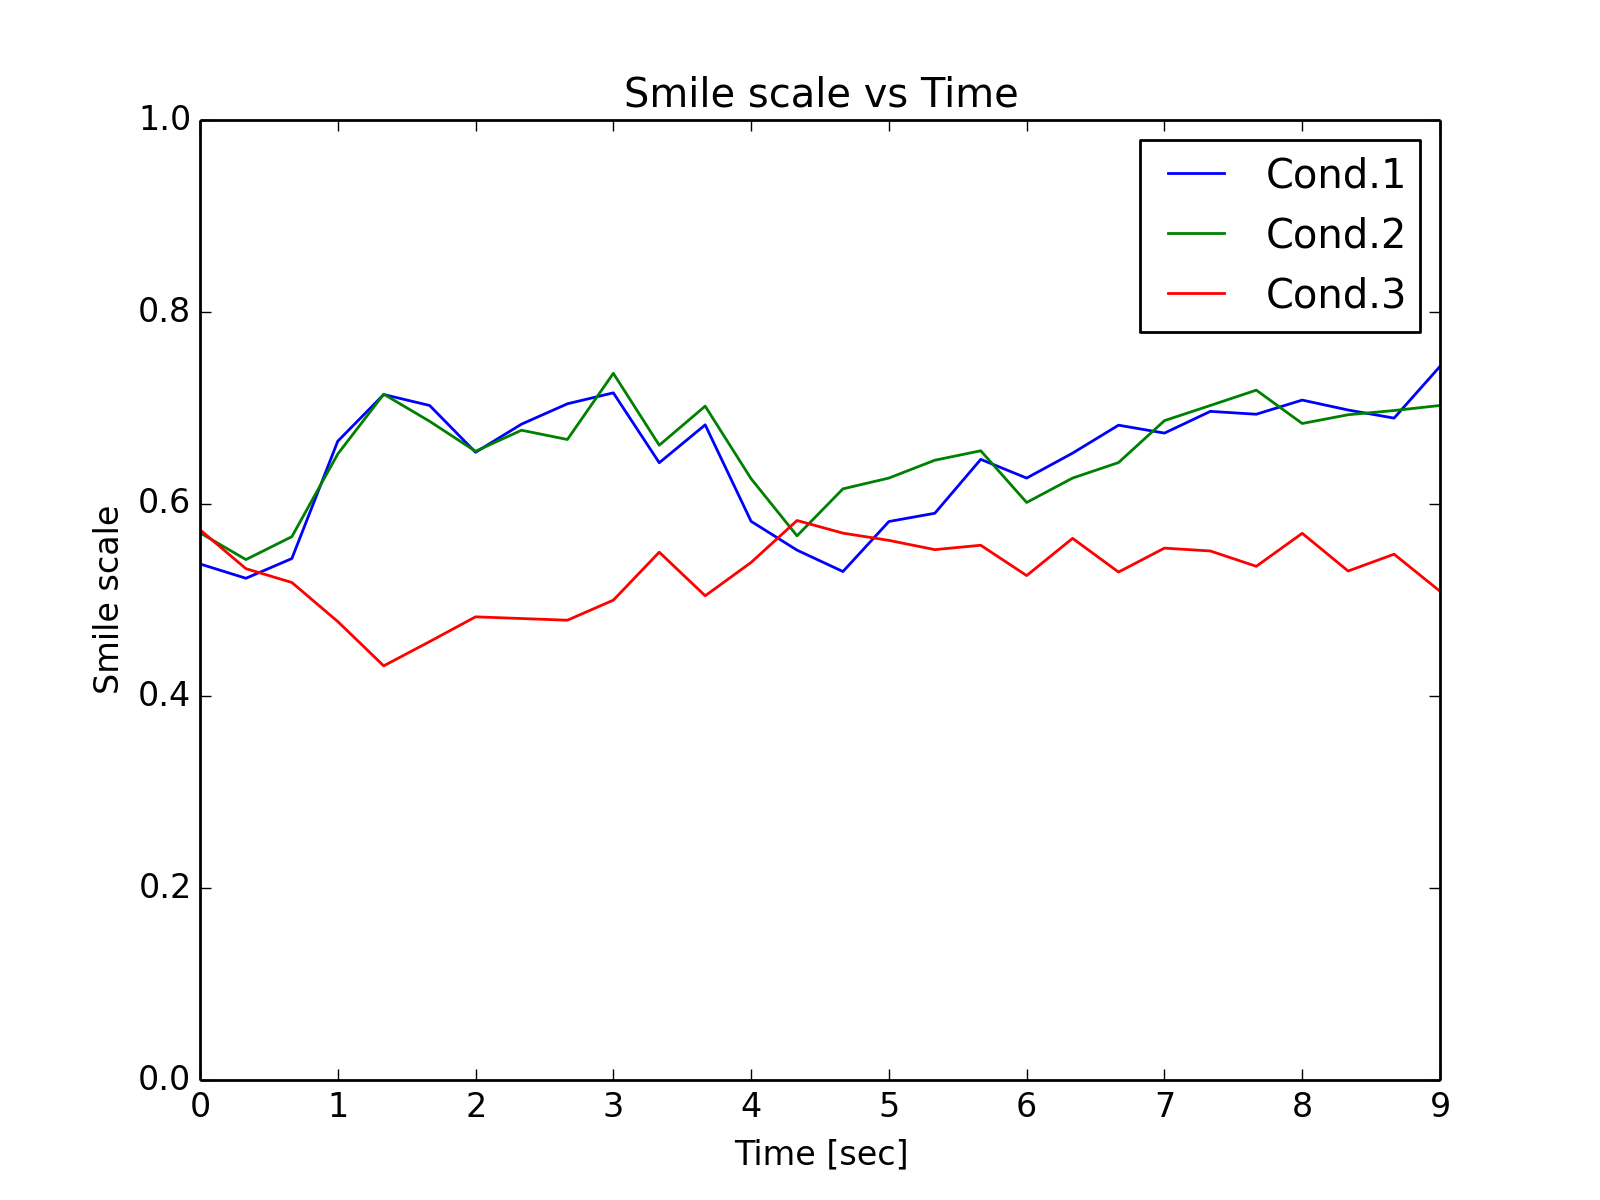
\includegraphics[width=90mm, bb=0 0 600 450]{images/smooth5_avg.png}
\caption{笑顔尺度の値の変化}
  \label{graph-smooth}
\end{figure}

\begin{figure}[h!]
  \centering  
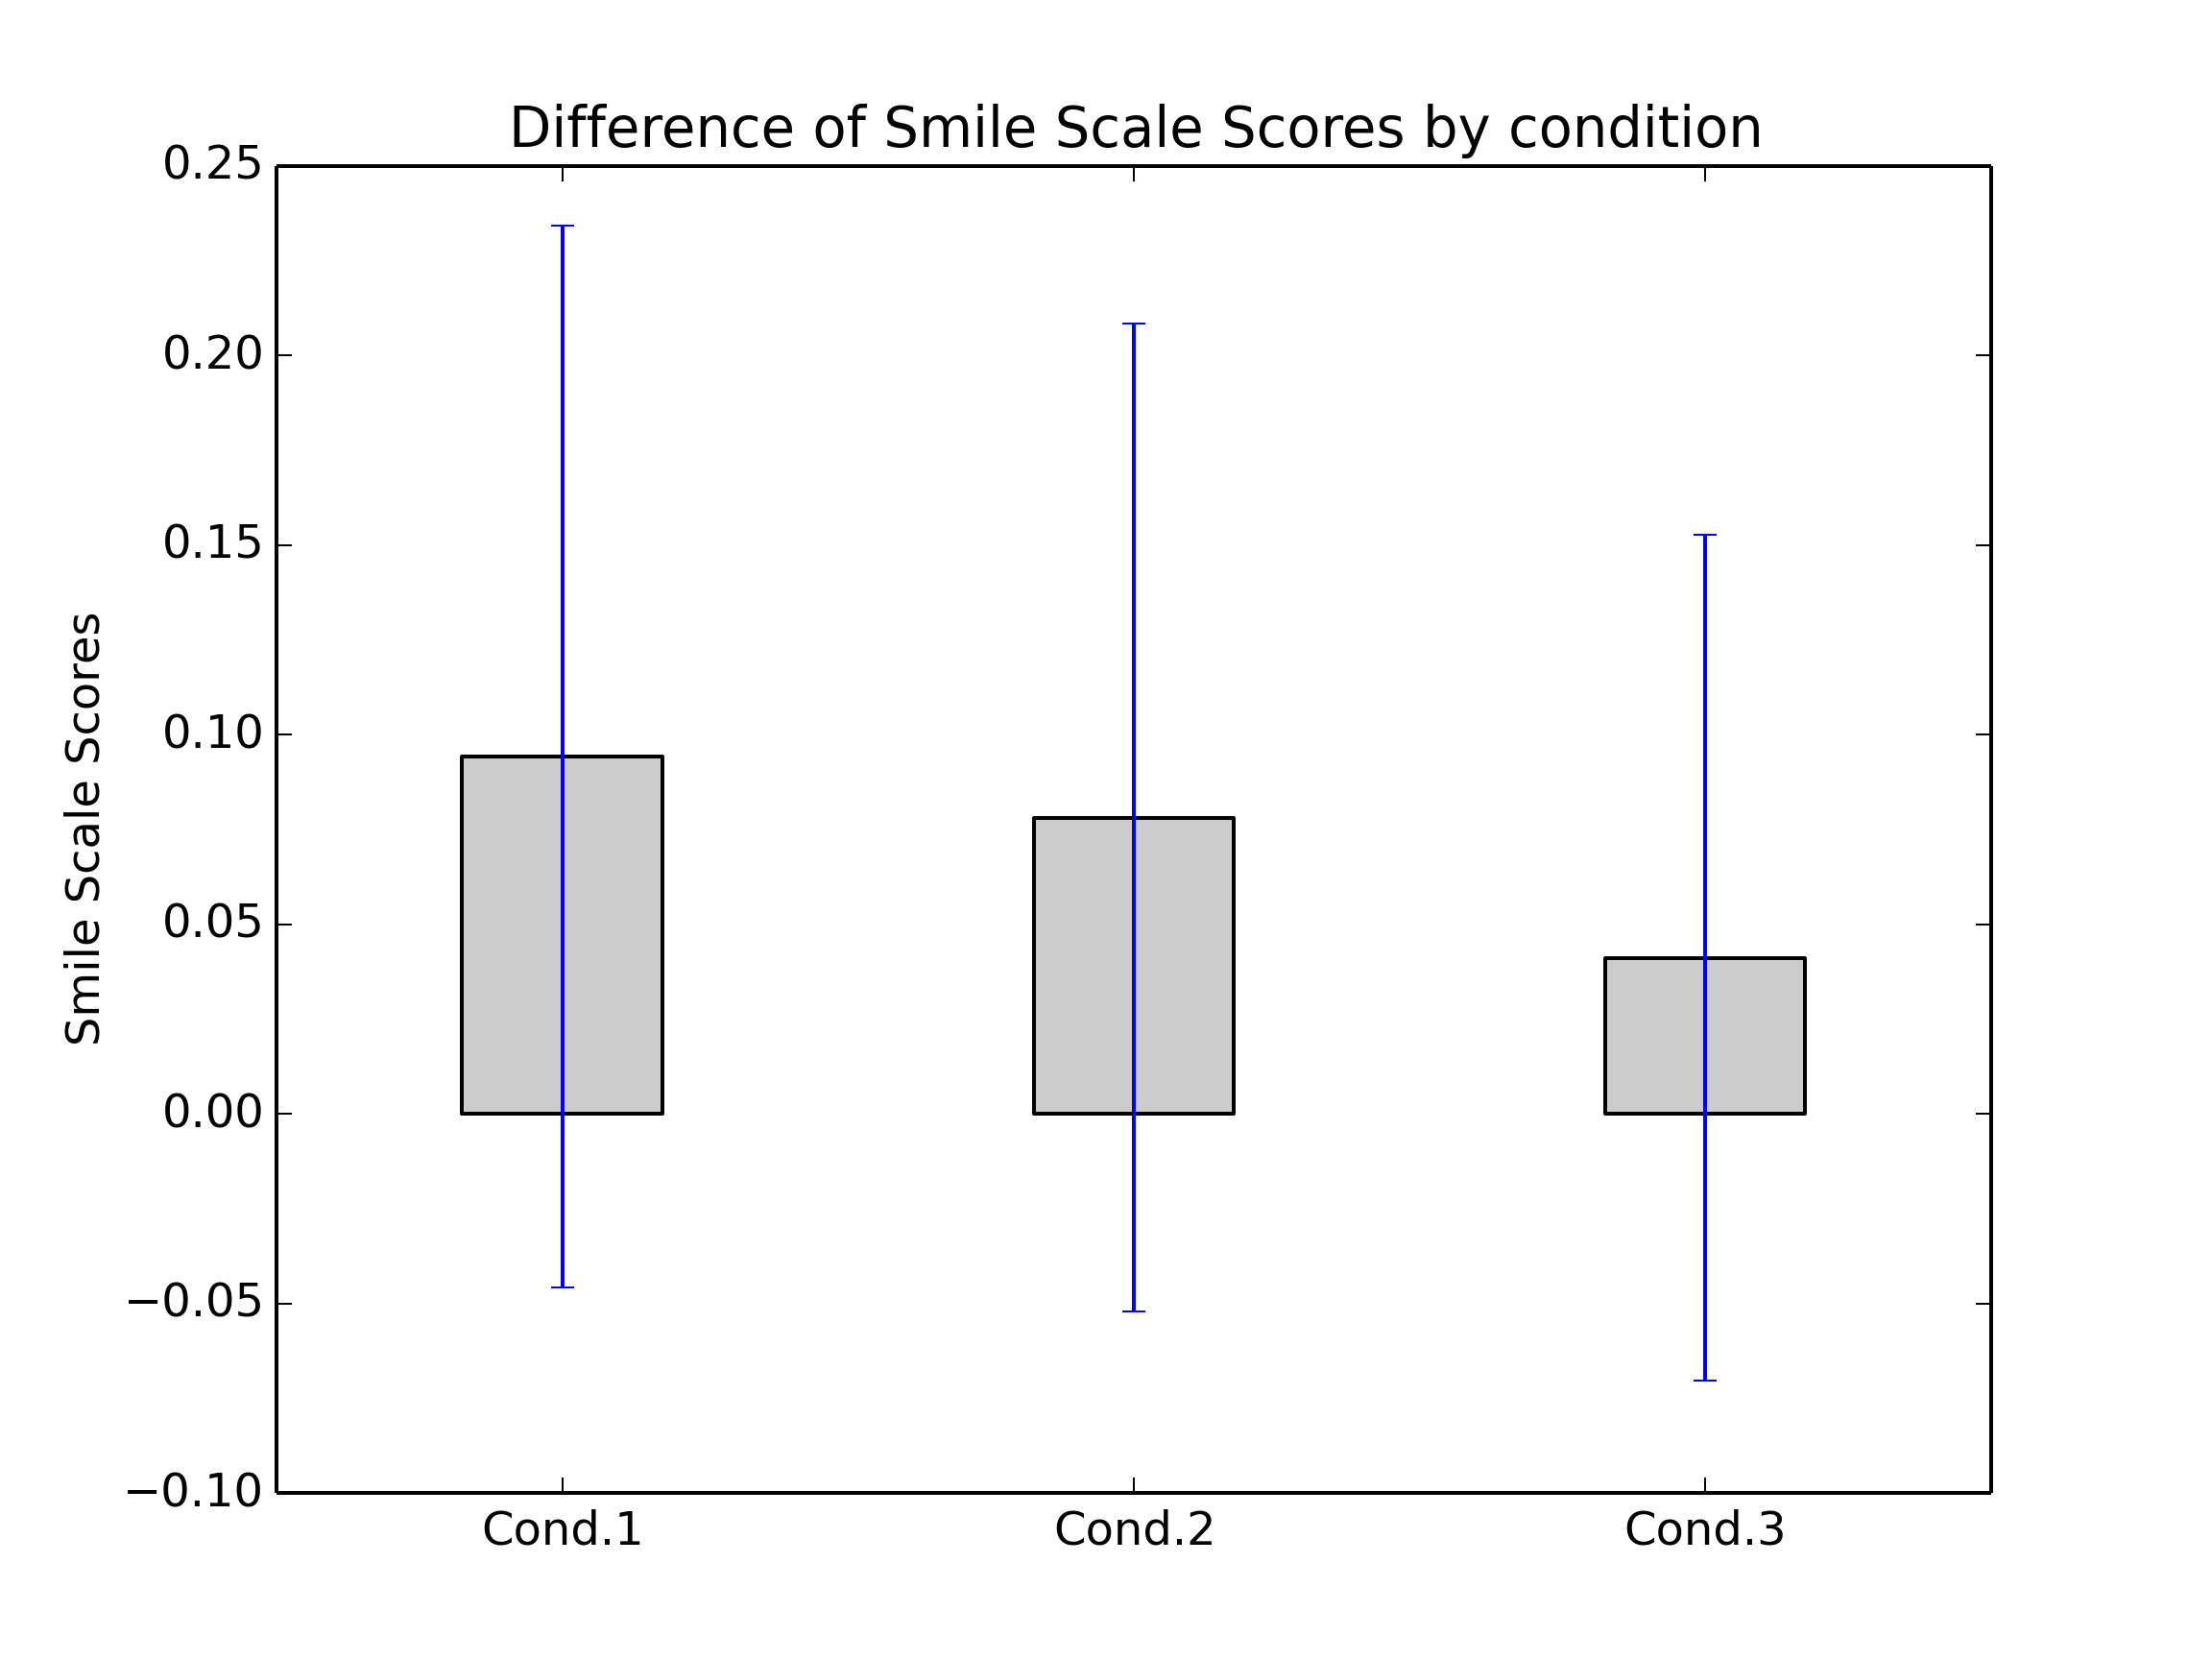
\includegraphics[width=90mm, bb=0 0 600 450]{images/graph-diff.png}
\caption{笑顔尺度の差の平均値}
  \label{graph-avg}
\end{figure}

実際に効果が出ていることを確かめるため,0.0秒〜1.0秒の笑顔度の値を作り笑いの笑顔の値,1.0〜2.0秒の笑顔度の値の平均値を音声によって誘発された笑顔の値の代表値として,条件内で作り笑い-誘発笑いの間に差があるかどうかウィルコクソンの符号順位検定を用いて検定した結果,作り笑い-誘発笑いの笑顔度の差は条件1,2で有意 ($p<.02$) だが,条件3では有意ではなかった.

さらに (誘発笑いの笑顔度) - (作り笑いの笑顔度) の差について,各条件群について対応あり3群の分散分析を行った結果,$p<0.05$で有意に差があるという結果が出た.2条件間で検定を行ったところ,条件1-条件3,条件2-条件3について有意に差があり,Bonferroniの補正を考慮しても条件2-条件3間では$p<0.05$で優位に差があった.

\begin{table}[htb]
  \begin{center}
    \caption{対応あり分散分析の結果 (p値, カッコ内は Bonferroni の補正)}
    \begin{tabular}{|l|c|r||r|} \hline
      3群 & $0.025$  \\ \hline 
      条件1-2 & $0.760 (2.280)$ \\ \hline
      条件2-3 & $0.004 (0.012)$ \\ \hline
      条件1-3 & $0.041 (0.123)$ \\ \hline
    \end{tabular}
    \label{tab:price}
  \end{center}
\end{table}


また,笑い誘発の男女差を確認するため,各条件の (誘発笑いの笑顔度) - (作り笑いの笑顔度) の値についての男女差を,マン・ホイットニーのU検定を用いて検定した結果を表\ref{manw}に示す.条件1 (青年の笑い声) については女性のほうが,条件3 (シャッター) については男性のほうが,それぞれ有意に笑顔が誘発されやすい(いずれも$p < .05$)という結果となった.

\begin{table}[htb]
  \begin{center}
    \caption{マン・ホイットニーのU検定の結果 (p値)}
    \begin{tabular}{|c|c|c|}  \hline
      条件1 (青年) & $0.037$ & (男性) $<$ (女性) \\ \hline
      条件2 (幼児)  & $0.156$ & (男性) $<$ (女性) \\ \hline
      条件3 (シャッター) & $0.046$ & (男性) $>$ (女性) \\ \hline
    \end{tabular}
    \label{manw}
  \end{center}
\end{table}


さらに,音声の種類の違いが笑顔誘発度合いに及ぼす影響の男女差を調べるため,各被験者について2条件間の誘発笑いの笑顔度の差について,男女差があるかを確認した.条件1(青年) の誘発笑いの笑顔度と,条件2(幼児)の誘発笑いの笑顔度の符号を考慮した差は,女性のほうが有意に大きい ($p < .05$)が
ほかの2条件間では男女差は見られなかった.これは,女性は比較的青年よりも幼児の笑い声に笑いを誘発され,男性はその逆の傾向があることを示唆する.

%結果を\ref{pair-genderdiff}に示す.

%\begin{table}[htb]
%  \begin{center}
%    \caption{マン・ホイットニーのU検定の結果 (p値)}
%    \begin{tabular}{|l|c|r||r|} \hline
%      (条件1) - (条件2) & $0.024$ & (男性) $>$ (女性) \\ \hline
%      (条件2) - (条件3) & $0.266$ & (男性) $<$ (女性) \\ \hline
%      (条件3) - (条件1) & $0.056$ & (男性) $>$ (女性) \\ \hline
%    \end{tabular}
%    \label{pair-genderdiff}
%  \end{center}
%\end{table}

最後に,代表的な画像を下記に示す.

\begin{figure}[h]
\begin{minipage}{0.49\columnwidth}
\begin{center}
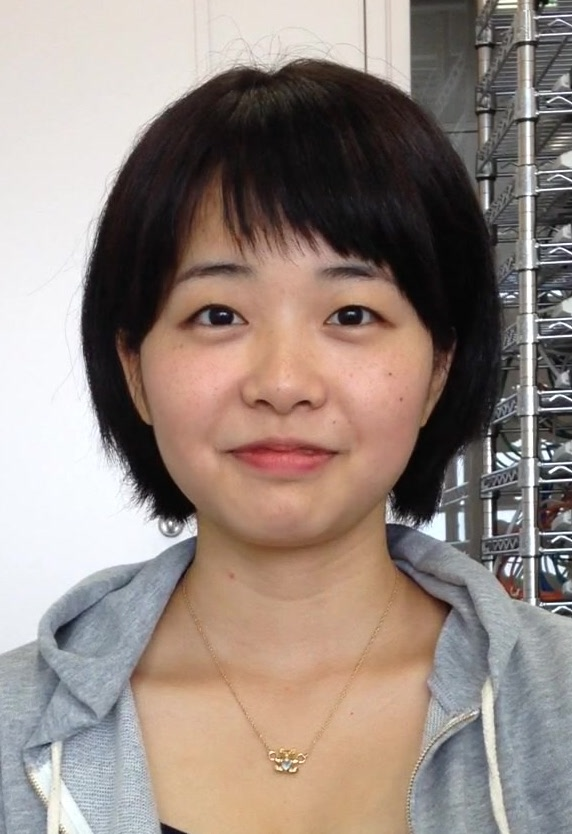
\includegraphics[width=35mm, bb=0 0 572 834]{images/cap_28.jpg}
\caption{条件2}
\end{center}
\end{minipage}
\begin{minipage}{0.49\columnwidth}
\begin{center}
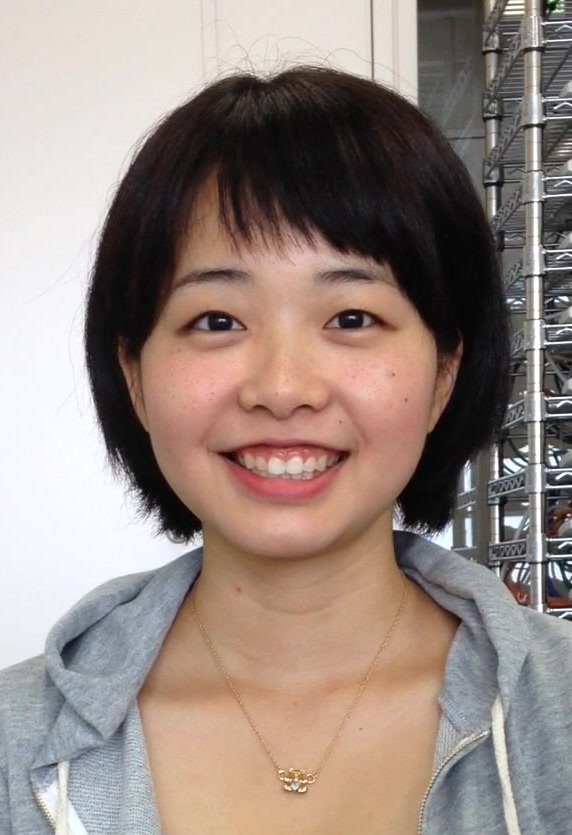
\includegraphics[width=35mm, bb=0 0 572 834]{images/cap_123.jpg}
\caption{条件3}
\end{center}
\end{minipage}
\end{figure}


\subsection{その他}

女性被験者3名から,男性の笑い声は不快だという意見があった.また女性の被験者2名から,男性青年の笑い声よりも赤ちゃんのほうが笑いやすいという意見があった.そのうち1名は,それは自分が女性だからではないかという意見を付した.これらの報告は,実際に女性では青年より幼児の方が笑顔度の誘発度合いが大きかったことと符合する.

また男性のうち2名は,「いつも写真に撮られるくらいの笑顔で映ってください」という教示に対し,「いつも写真には笑顔では映らない」と応えたため,「それでは,いつも写真に取られる表情で写ってください」と指示した.今回の実験では,このような被験者に対する対応は準備していなかった.

\subsection{まとめ}

本システムにおいて,条件1(青年笑い声),条件2(幼児笑い声)で笑顔を誘発できていること,さらに対照とした条件3ではその効果が現れないことを検証した.さらに男女差を分析した.また,男性青年の笑い声よりも幼児の笑い声のほうが笑顔を誘発しやすい傾向が女性では強かった.

また,笑顔の誘発にはディレイが存在し,誘発された笑顔が最も顕著になるのは条件1, 条件2ともに音声再生からおよそ1.5秒後であることがわかった.写真撮影システムを構築する場合は,この結果を元にシャッターを切る時間を設定すれば良い.ただし,この値は再生する音声によって大きく異なるだろうから,異なる音声を扱う場合には今回のような実験を繰り返す必要がある.

比較可能な尺度としてRekognition APIの笑顔尺度を利用した.Rekognition を公開しているOrbeus社は,顔認識エンジン専業の企業で,多数の企業に顔認識システムを提供している.ただし,笑顔度分析の科学的基礎づけは公開されておらず,この値の信頼性に対して評価を加えることは難しい.しかし連続した表情の変化に対して,ほぼ連続した値が得られていることから,ある程度信頼できるものと考えられる.

\section{実験2}

\subsection{目的}

実験1では,3種類の音声を呈示しながら撮影した写真についてコンピュータビジョンの技術を使って笑顔尺度を測定し,この値を比較することで,我々のシステムが有効に笑顔を誘発できていることが分かった.しかし実験1だけでは,今回構築したカメラシステムが我々の考える「自然な笑顔」であることはわからない.

\subsection{実験条件および実験設備環境}

node.js を用いてWebサーバを構築した.評価者は各々のPCのWebブラウザを通じて評価実験に参加した.画面の大きさの条件などは統制できなかったが,ウインドウを最大化してから実験を進めるように指示した.

評価者

\subsection{手続き}

被験者は,割り当てられた写真2枚の組について,どちらが自然な笑顔であるかを判定した.割り当てられた写真は同じ人物の,顔全体・鼻より上・鼻より下の3パターンがあった.

本実験では,非撮影者とは異なる評価者に撮影された画像を見せ,笑顔の自然さを評価させることで,我々のシステムが自然な笑顔を誘発できているかどうかを検証することを目的とする.



\begin{thebibliography}{10}

\end{thebibliography}



%\pagebreak%%!!!
%\vspace*{-\baselineskip}%%!!!

%\appendix
%7
%\section{付録の書き方}

%付録がある場合には,参考文献リストの直後にコマンド \|\appendix| に引き続
%いて書く.付録では,\|\section| コマンドが{\bf A.1},{\bf A.2}などの見出
%しを生成する.

%7.1
%\subsection{見出しの例}

%付録の \|\subsetion| ではこのよう見出しになる.

%8
%\section{研究会論文用コマンド}
%\label{sig}

%各研究会論文誌(トランザクション)には各々に固有のサブタイトル,略称,通
%番がある.最終原稿では,以下のコマンドを \|\documentclass| の{\bf オプショ
%ン}とすることで,これらの情報を与える.

%\begin{itemize}
%\item \|PRO|(プログラミング)
%\item \|TOM|(数理モデル化と応用)
%\item \|TOD|(データベース)
%\item \|ACS|(コンピューティングシステム)
%\item \|CDS|(コンシューマ・デバイス\,\&\,システム)
%\item \|TBIO|(Bioinformatics)\footnote{%
%TBIO, SLDM, CVAは英文論文誌であるので和名はない.}
%\item \|SLDM|(System LSI Design Methodology)\footnotemark[5]
%\item \|CVA|(Computer Vision and Applicaitons)\footnotemark[5]
%\end{itemize}

%また英文論文作成の際には \|english| をオプションに追加すればよい.したがっ
%て,\|\documentclass[PRO]{ipsj}| とすれば「プログラミング」の和文用,
%\|\documentclass[PRO,english]| \|{ipsj}| とすれば英文用となる.

%また研究会には「号」と連動しない「発行月」があるため,学会あるいは編集委
%員会の指示に基づき,発行月を
%
%\begin{itemize}\item[]
%\|\setcounter{|{\bf 月数}\|}{<発行月>}|
%\end{itemize}
%
%によって指定する.

%この他,以下の各節で示すように,いくつかの論文誌に固有の機能を実現するた
%めのコマンドなどが用意されている.

%\newpage%%

%9
%\section{各分冊固有コマンド}

%各分冊によってそれぞれ細かい仕様が違うため,同じコマンドでも出力結果が異
%なる場合がある.また「再受付」,「再々受付」が入る場合があり,それらは

%\noindent
%和文では
%\begin{itemize}\item[]
%\|\|{\bf 再受付}\|{<年>}{<月>}{<日>}|\\
%\|\|{\bf 再再受付}\|{<年>}{<月>}{<日>}|
%\end{itemize}
%英文では
%\begin{itemize}\item[]
%\|\|{\bf rereceived}\|{<年>}{<月>}{<日>}|\\
%\|\|{\bf rerereceived}\|{<年>}{<月>}{<日>}|
%\end{itemize}
%とプリアンブルに追加する.

%9.1
%\subsection{\<「プログラミング(PRO)」固有機能}

%\<「論文誌:プログラミング」には論文以外に,プログラミング研究会での研究
%発表の内容梗概が含まれている.この内容梗概は,\|\documentclass|のオプショ
%ンとして\|abstract|を指定する.\ref{config}~節の\|\maketitle|までの内容
%からなるファイル(すなわち本文がないファイル)から生成する.なお\|\|{\bf 
%受付}や\|\|{\bf 採録}は不要であるが,代わりに発表年月日を,

%\noindent
%和文では
%\begin{itemize}\item[]
%\|\|{\bf 発表}\|{<年>}{<月>}{<日>}|
%\end{itemize}
%英文では
%\begin{itemize}\item[]
%\|\|{\bf Presents}\|{<年>}{<月>}{<日>}|
%\end{itemize}
%により指定する.

%9.1
%\subsection{\<「データベース(TOD)」固有機能}

%\<「論文誌:データベース」の論文の担当編集委員は,
%\begin{itemize}\item[]
%\|\Editor{<氏名>}|
%\end{itemize}
%により指定する.和文では「担当編集委員」,英文では「Editor in Charge:」
%と入る.

%またスタイルの変更に伴い,\underline{本文の最後}に入るので,
%\|\end{document}|の前に直接置く.

%9.2
%\subsection{\<「コンシューマ・デバイス\,\&\,システム(CDS)」固有機能}

%\<「論文誌:コンシューマ・デバイス\,\&\,システム」では,
%論文の種類によって見出しが変わるため,
%オプションで切替えを行う.

%各種別は
%\begin{itemize}
%\item \|systems  |コンシューマ・システム論文\\
%\|         |Paper on Consumer Systems

%\item \|services |コンシューマ・サービス論文\\
%\|         |Paper on Consumer Services

%\item \|devices  |コンシューマ・デバイス論文\\
%\|         |Paper on Consumer Devices

%\item \|research |研究論文\\
%\|         |Research Paper
%\end{itemize}
%となる.

%和文のコンシューマ・システム論文なら,\\
%\|\documentclass[CDS,systems]{ipsj}|
%となり,英文原稿なら \|english|を追加すればよい.

%9.3
%\subsection{\<「Bioinformatics(TBIO)」固有機能}

%Trans.\ Bioinformatics (TBIO)は英文論文誌であるので,\|TBIO|オプションの
%指定によって自動的に\|english|オプションが指定されたものとみなされ,
%\|english| オプションの省略が可能.

%論文種別は以下の3種.
%\begin{itemize}
%\item \makebox[4.9zw][l]{指定なし} Original Paper (Default)
%\item \|Data     | Database/Software Paper
%\item \|Survey   | Survey Paper
%\end{itemize}

%\|\documentclass[TBIO]{ipsj}|でOriginal Paper,\\
%\|\documentclass[TBIO,Survey]{ipsj}|でSurvey Paperとなる.

%また,担当編集委員はTOD同様,\|\Editor|で定義するが,「Communicated by」
%となる.TOD同様,\|\end{document}|の前に直接置く.

%9.4
%\subsection{\<「Computer Vision and Applicaitons\\\<(CVA)」固有機能}

%Trans.\ CVAも英文論文誌であるため,\|english| オプションの省略が可.

%論文種別は3種類あり,
%\begin{itemize}
%\item \makebox[4.9zw][l]{指定なし} Regular Paper (Default)
%\item \|Research | Research Paper
%\item \|system   | Systems Paper
%\end{itemize}
%となる.

%TBIO同様,担当編集委員が入り,
%挿入文章もTBIO同様,「Communicated by」となる.

%9.5
%\subsection{\<「System LSI Design Methodology(SLDM)」固有機能}

%Trans.\ SLDMも英文論文誌であるため,\|english| オプションの省略が可.

%論文種別は2種類あり,
%\begin{itemize}
%\item \makebox[4.9zw][l]{指定なし} Regular Paper (Default)
%\item \|Short    | Short Paper
%\end{itemize}
%となる.

%SLDMも担当編集委員が入るが挿入文章が論文によって自動挿入文章が異なる.

%通常は「Recommended by Associate Editor:」,\|invited|のオプションが入っ
%た場合のみ,「Invited by Editor-in-Chief:」となる.



%% 以下は無視されます

\begin{biography}
\profile{m}{情報 太郎}{1970年生.1992年情報処理大学理学部情報科学科卒.
1994年同大大学院修士課程了.同年情報処理学会入社.オンライン出版の研究
に従事.電子情報通信学会,IEEE,ACM 各会員}
%
\profile{n}{処理 花子}{1960年生.1982年情報処理大学理学部情報科学科卒.
1984年同大大学院修士課程了.1987年同博士課程了.理学博士.1987年情報処
理大学助手.1992年架空大学助教授.1997年同大教授.オンライン出版の研究
に従事.2010年情報処理記念賞受賞.電子情報通信学会,IEEE,IEEE-CS,ACM
各会員}
%
\profile{s}{学会 次郎}{1950年生.1974年架空大学大学院修士課程了.
1987年同博士課程了.工学博士.1977年架空大学助手.1992年情報処理大学助
教授.1987年同大教授.2000年から情報処理学会顧問.オンライン出版の研究
に従事.2010年情報処理記念賞受賞.情報処理学会理事.電子情報通信学会,
IEEE,IEEE-CS,ACM 各会員}
%
\end{biography}



\end{document}
